% ML4H 2026 review manuscript
% Compile from this directory with:
%   latexmk -C
%   latexmk -pdf -interaction=nonstopmode -halt-on-error main.tex
%
% Keep the official jmlr.cls and jmlrutils.sty files unchanged.
% Confirm the submission track and institutional IRB wording before submission.

\documentclass[pmlr,twocolumn,10pt]{jmlr}

\mlhtrack{proceedings}

\newif\iffinal
\finalfalse
% \finaltrue

\iffinal
  \ifmlhneedspmlr
    \jmlrvolume{XXX}
    \jmlryear{2026}
  \fi
  \ifmlhfindings \jmlrproceedings{}{ML4H 2026 - Findings Track}\fi
  \ifmlhdemo     \jmlrproceedings{}{ML4H 2026 - Demo Track}\fi
  \jmlrworkshop{Machine Learning for Health (ML4H) 2026}
\else
  \jmlrproceedings{}{Submitted to ML4H 2026: \mlhtrackname}
  \jmlrworkshop{Machine Learning for Health (ML4H) 2026}
\fi

% Packages used by the official template.
\urlstyle{same}
\usepackage{booktabs}
\usepackage[switch]{lineno}

% Sparse line numbering preserves review usability without crowding the
% two-column layout. Remove \linenumbers in the camera-ready version.
\renewcommand\linenumberfont{\normalfont\tiny\sffamily}
\setlength\linenumbersep{7pt}
\modulolinenumbers[5]

\title[Who Can Be Scored?]{Who Can Be Scored? Cohort Availability Limits
Population-Level Capture in Prenatal Risk Triage}
\author{Anonymous Author(s)}

\begin{document}

\maketitle
\linenumbers

\ifmlhdemo\else
\begin{abstract}
Clinical risk models are often evaluated only among individuals for whom a
prediction can be generated, obscuring events outside the scoreable cohort.
Using U.S. CDC Natality records, we fitted one LightGBM model per outcome on
2022 singleton births and evaluated preterm delivery, neonatal intensive care
unit admission, and low birth weight on a 2023 temporal test. Early
eligibility, defined as prenatal-care initiation in months 1--3, covered
approximately 74.7\% of records but only 69.4--71.8\% of outcome events. At
an equal absolute referral budget of 10\% of each target-specific population,
the early policy captured 2.58, 2.73, and 3.43 percentage points fewer events
than the full-cohort policy, corresponding to 7,821, 8,271, and 8,356 events.
Paired full-size bootstrap intervals from 500 replicates were above zero for
all outcomes. Clinical prediction evaluation should therefore distinguish
scoreability ceiling, conditional recall, and population event capture under
an explicit resource budget.
\end{abstract}

\begin{keywords}
clinical risk prediction; cohort eligibility; scoreability; prenatal care;
resource-constrained triage; temporal evaluation
\end{keywords}
\fi

\ifmlhneedsstatements
\paragraph*{Data and Code Availability}
The study uses publicly available, de-identified CDC Natality public-use
records. The review package will include anonymized preprocessing and analysis
code, locked configurations, input hashes, and article-facing result tables.
A de-anonymized repository will be released after review.

\paragraph*{Institutional Review Board (IRB)}
The analysis used publicly available, de-identified public-use records and
involved no participant interaction or access to identifiable information.
The applicable institutional determination will be provided if the paper is
accepted.
\fi

\section{Introduction}
\label{sec:intro}

Clinical prediction can fail at two stages. A person may be unavailable for
scoring because the required encounter or measurement has not occurred, or a
model may rank an available case incorrectly. Standard discrimination and
within-cohort recall primarily address the second stage and do not count
events outside the scoreable cohort.

This distinction is consequential in prenatal triage. A policy restricted to
people initiating prenatal care early cannot act on later-entry, no-care, or
unknown-timing records. Conventional top-$k$ comparisons can also confound
eligibility with capacity when $k$ is defined separately in cohorts of
different sizes. We therefore compare early-entry and full-cohort policies
while holding the fitted model, prediction vector, and absolute referral
budget fixed.

Prior work treats nonrandom observation, post-score abstention, and finite
clinical capacity largely as separate problems. Informative-presence studies
show that observed EHR cohorts can differ systematically from target
populations \citep{haneuse2016selection,sisk2021informative}.
Selective-prediction methods abstain after the required inputs reach the model
\citep{leibig2017uncertainty}, whereas resource-constrained
evaluation can impose an absolute capacity among already scored candidates
\citep{singh2023resource}. Prenatal studies have used gestational landmarks or
national vital-statistics cohorts
\citep{osterman2026prenatal,abraham2022dense,schulz2022delivery},
but generally report performance within records meeting each study's
inclusion and data-availability criteria. In our targeted audit, we found no
study that retained events outside the scoreable cohort in the population
denominator while fixing both the model and the absolute referral budget.

\begin{figure*}[t]
\floatconts
  {fig:study-design}
  {\caption{Fixed-model, equal-budget study design. One outcome-specific
  LightGBM model is fitted using CDC 2022, applied once to the CDC 2023
  temporal test, and evaluated under early-entry and full-cohort eligibility.
  Both policies select the same absolute number of records. Events in groups
  unavailable to the early policy remain in the full-population denominator.}}
  {\centering
   
\includegraphics[width=0.985\textwidth]{figures/figure1_study_design}}
\end{figure*}

\section{Methods}
\label{sec:methods}

\paragraph{Data and population.}
CDC Natality 2022 contained 3,676,029 records and was used for model
development and internal held-out evaluation. CDC 2023 contained 3,605,081
records and was used only as a temporal test. The primary population comprised
U.S.-resident singleton births with a known outcome value.

\paragraph{Outcomes and eligibility.}
Outcomes were preterm delivery (obstetric-estimate gestational age below 37
weeks), neonatal intensive care unit (NICU) admission, and low birth weight
(LBW; below 2,500~g). Early eligibility required prenatal-care initiation in
months 1--3. Later entry, no prenatal care, and unknown timing remained in the
full-population denominator but were unavailable to the early policy. Source
code 99 and blank prenatal-care-month values were mapped to missing; 0 was
retained as no prenatal care.

\paragraph{Fixed-model comparison.}
For each outcome, one LightGBM model was fitted on CDC 2022 using the
pre-specified \texttt{booking\_strict} features (350 trees, learning rate
0.05, 31 leaves, and \texttt{min\_child\_samples}=100). We used no class
weighting, oversampling, or hyperparameter optimization. Both policies used
the same fitted model and the same CDC 2023 prediction vector.

For target-specific full-population size $N_{\mathrm{full}}$, the absolute
budget was
\[
B=\operatorname{round}(qN_{\mathrm{full}}),
\qquad q\in\{0.05,0.10\}.
\]
Each policy selected the top $B$ risks within its eligible set. Let
$E_{\mathrm{full}}$ be all population events, $E_{\mathrm{early}}$ events in
the early cohort, and $\mathrm{TP}_{s}(B)$ events captured by policy $s$. We
report
\begin{align*}
\mathrm{Ceiling} &= \frac{E_{\mathrm{early}}}{E_{\mathrm{full}}},\\
\mathrm{Recall}_{s} &= \frac{\mathrm{TP}_{s}(B)}{E_s},\\
\mathrm{Capture}_{s} &= \frac{\mathrm{TP}_{s}(B)}{E_{\mathrm{full}}}.
\end{align*}
The primary estimand was full-minus-early population event capture.

\paragraph{Uncertainty and supporting analyses.}
We used 500 paired, full-size, record-level bootstrap replicates with
identical multiplicities for both policies and reconstructed top-$B$
selection in every replicate. Percentile intervals were computed for the
full-minus-early difference. At the 10\% budget, true positives were
decomposed by care-entry group. Platt calibration was fitted on CDC 2022 and
evaluated on held-out 2022 and temporal-test 2023 data. We also repeated the
analysis among all U.S.-resident births; this remained sensitivity evidence
because pregnancy-level clustering could not be reconstructed.


\begin{figure*}[t]
\floatconts
  {fig:fixed-budget-capture}
  {\caption{Population event capture under equal absolute referral budgets.
  Circles show early-entry eligibility and squares show full-cohort
  eligibility. Connecting segments show the change in captured population
  events; labels report the full-minus-early difference with its paired 95\%
  bootstrap interval and the number of additional events.}}
  {\centering
   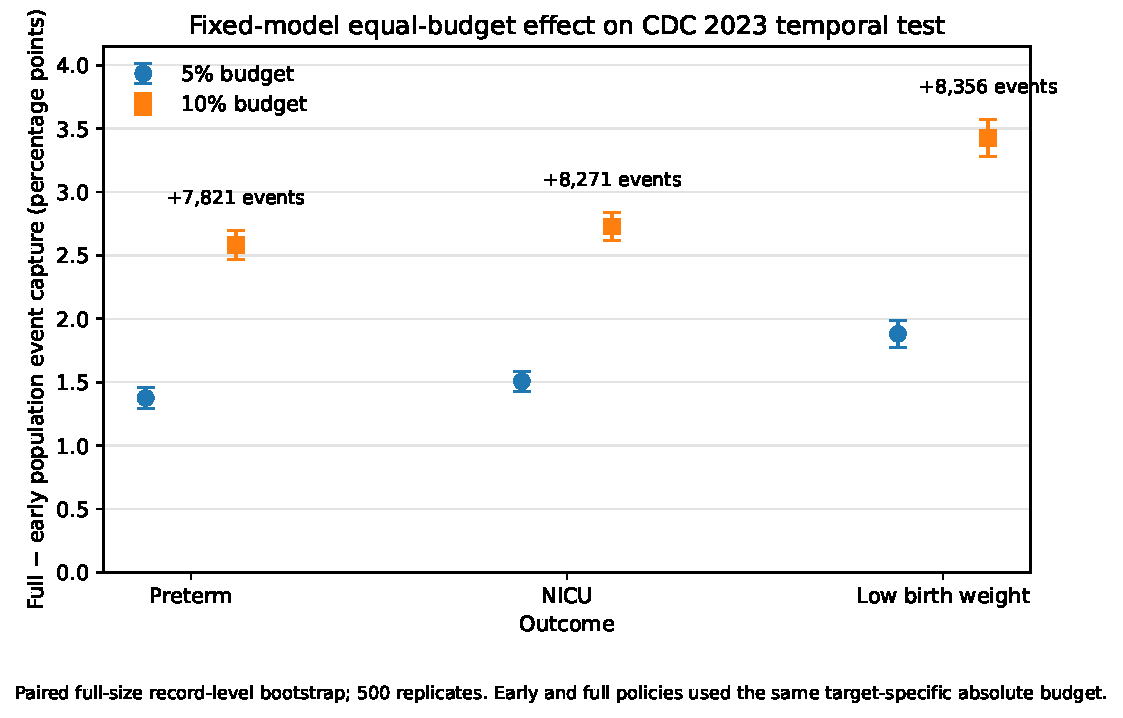
\includegraphics[width=0.97\textwidth]{figures/figure2_fixed_budget_capture}}
\end{figure*}

\section{Results}
\label{sec:results}

\paragraph{Availability imposed an event ceiling.}
Early eligibility covered 74.71--74.73\% of CDC 2023 records but only 71.83\%
of preterm events, 70.62\% of NICU admissions, and 69.39\% of LBW events
(Table~\ref{tab:main-results}). Thus, 28--31\% of events were outside the
early-scoreable cohort before classifier error was considered.

\paragraph{Full eligibility increased capture at equal capacity.}
At the 10\% budget, full-cohort capture exceeded early-entry capture by 2.58,
2.73, and 3.43 percentage points for preterm delivery, NICU admission, and
LBW, representing 7,821, 8,271, and 8,356 additional events. At 5\%, gains
were 1.38, 1.51, and 1.88 points (Figure~\ref{fig:fixed-budget-capture}). Full
precision was also higher at the equal 10\% budget: 18.64\% versus 16.39\% for
preterm delivery, 17.88\% versus 15.50\% for NICU admission, and 16.80\%
versus 14.40\% for LBW.



\begin{table*}[t]
\floatconts
  {tab:main-results}
  {\caption{CDC 2023 temporal-test results at the target-specific 10\%
  absolute referral budget. Capture is population event capture; intervals
  are paired bootstrap percentile intervals from 500 replicates.}}
  {\centering
  \scriptsize
  \setlength{\tabcolsep}{2.9pt}
  \resizebox{\textwidth}{!}{%
  \begin{tabular}{lrrrrrrrrr}
  \toprule
  Outcome &
  \shortstack{Full\\$N$} &
  \shortstack{Early\\$N$ (\%)} &
  \shortstack{Events\\$n$ (\%)} &
  \shortstack{Event\\ceiling} &
  \shortstack{Budget\\$B$} &
  \shortstack{Early\\capture} &
  \shortstack{Full\\capture} &
  \shortstack{$\Delta$ capture, pp\\(95\% CI)} &
  \shortstack{Additional\\TP} \\
  \midrule
  Preterm delivery & 3{,}480{,}382 & 2{,}601{,}060 (74.73) &
  303{,}001 (8.71) & 71.83 & 348{,}038 & 18.83 & 21.41 &
  2.58 (2.47--2.70) & 7{,}821 \\
  NICU admission & 3{,}476{,}584 & 2{,}597{,}274 (74.71) &
  303{,}285 (8.72) & 70.62 & 347{,}658 & 17.77 & 20.50 &
  2.73 (2.62--2.84) & 8{,}271 \\
  Low birth weight & 3{,}480{,}316 & 2{,}600{,}093 (74.71) &
  243{,}776 (7.00) & 69.39 & 348{,}032 & 20.56 & 23.98 &
  3.43 (3.28--3.57) & 8{,}356 \\
  \bottomrule
  \end{tabular}}}
\end{table*}

\paragraph{Uncertainty was consistently positive.}
All CDC 2023 intervals were above zero. At 10\%, intervals were 2.47--2.70
points for preterm delivery, 2.62--2.84 for NICU admission, and 3.28--3.57
for LBW. Held-out CDC 2022 produced similar differences of 2.60, 2.59, and
3.12 points, respectively, with intervals of 2.26--2.98, 2.29--2.95, and
2.65--3.62 points.

\paragraph{Gains arose outside the early cohort.}
At 10\%, full eligibility gained 22,271 preterm, 20,557 NICU, and 21,857 LBW
true positives from later-entry, no-care, and unknown-timing groups. The same
budget reallocation reduced true positives within months 1--3 by 14,450,
12,286, and 13,501, producing the net gains above.

\paragraph{Supporting analyses were consistent.}
Raw CDC 2023 full-cohort models had calibration intercepts from $-0.019$ to
$0.015$ and slopes from 0.995 to 0.998; Platt scaling did not improve Brier
score. All-birth 10\% differences remained positive at 2.18, 2.51, and 2.85
points for preterm delivery, NICU admission, and LBW.

\FloatBarrier

\section{Discussion}
\label{sec:discussion}

Restricting scoring to prenatal-care entry in months 1--3 reduced population
capture after fixing the model, predictions, and absolute budget. The result
is not a claim about a superior architecture: eligibility determines which
events are available for selection. It also differs from selective
prediction, which abstains after a scoreable case reaches the model. Here,
events outside the early cohort remain in the denominator because they remain
part of the population the triage policy is intended to serve.

The mechanism analysis showed the operational trade-off. Full eligibility
reallocated the same referral capacity from some early-entry records toward
high-risk later-entry, no-care, and unknown-timing records. Gains outside the
early cohort exceeded losses within it for all outcomes.

Limitations include retrospective administrative data, non-optimized 5\% and
10\% capacity scenarios, temporal rather than cross-system evaluation, and no
causal interpretation of care entry. Multiple-birth records may be dependent,
and pregnancy-level clustered uncertainty was unavailable. Secondary
\texttt{pregnancy\_oracle} variables were not reliably available at the early
clinical landmark and are not presented as deployable inputs.

Clinical triage evaluations should separately report scoreability ceiling,
conditional performance among eligible records, and population event capture
under an explicit absolute budget.

\iffinal
\acks{Acknowledgments will be added only to the camera-ready manuscript.}
\fi

\nolinenumbers
\begingroup
\small
\setlength{\bibsep}{2pt}
\bibliography{references}
\endgroup

\end{document}
